\documentclass[11pt]{article}
\usepackage{graphicx}

\title{NRR-Guarantee: Bounded Commit/Defer Guarantees Under Explicit Conditions}
\author{Kei Saito}
\date{March 21, 2026}

\begin{document}
\maketitle

\begin{abstract}
This manuscript sets the current downstream \texttt{Guarantee} surface for the
Non-Resolution Reasoning (NRR) program. Its purpose is to close the next paper
as a bounded claim layer rather than as a broad universality paper. Under
explicit provider, family, horizon, and observability conditions, the current
manuscript integrates two supported claim surfaces and one downstream-
acceptance surface that closes as a two-provider mixed result: frozen early
ambiguity-turn resolution, repaired Phase 2 downstream acceptance, and repaired
first-step side-topic/quarantine workstart. On the current tested-provider
surface, the early ambiguity-turn \texttt{appropriate} read moves from
\texttt{0 / 24} to \texttt{24 / 24} on both providers, the repaired
downstream-acceptance read closes as a two-provider mixed result
(\texttt{Anthropic = inconclusive}, \texttt{Gemini = support}), and the
repaired first-step side-topic surface reaches \texttt{12 / 12} on both
providers. It also states the current later-horizon limit as explicit
failure-boundary reporting rather than as an additional guarantee. The result
is a narrow downstream paper surface for bounded guarantee claims. Across the
current Guarantee-owned sequence, the honest read is therefore staged rather
than uniform: Phase 1 remains provider-first \texttt{non-support}, while
Phase 2 closes as a two-provider mixed result rather than as pair-wide
support.
\end{abstract}

\section{Introduction}

NRR is not an anti-LLM framework. NRR does not replace standard LLM use. NRR
optimizes when to commit and when to defer, under explicit conditions.

Related work in mixed-initiative and task-oriented dialogue has long examined
adaptive initiative control and goal-oriented interaction management
~\cite{chucarroll2000mimic,saito2017taskdialogue}, while clarification-focused lines
study how a system should ask follow-up questions when a user's request remains
ambiguous or underspecified~\cite{deboni2003clarification,rao2018evpi,hu2020interactive}. Grounding-oriented work further emphasizes that dialogue systems
must recover collaboratively when interpretation is not yet fixed
~\cite{benotti2021groundedclarifications,benotti2021grounding}.

Within the NRR series, \texttt{Core} and \texttt{Phi} fixed the upstream
position-dependent identity and state-mapping surfaces~\cite{saito2025nrr,saito2026phi}.
\texttt{IME}, \texttt{Transfer}, \texttt{Coupled}, \texttt{Principles},
\texttt{Boundary}, and \texttt{Energy} then progressively constrained the
interface, transfer, dependency, efficiency, paired-effect, and downstream
boundary surfaces that the present manuscript inherits~\cite{saito2026ime,saito2026transfer,saito2026coupled,saito2026principles,saito2026boundary,saito2026energy}.

The current downstream architecture is \textit{Guarantee-centered}: \texttt{Policy},
\texttt{Dynamics}, and \texttt{Policy-Verification} are supporting layers for the
\texttt{Guarantee} line rather than independent completion targets. Accordingly, the
purpose of this manuscript is to close a bounded downstream paper that absorbs those
layers as constrained inputs.

The Core-to-Guarantee program goal itself is not being rewritten here. What the
series must establish from \texttt{Core} through \texttt{Guarantee} remains the
same: a framework grounded in position-dependent identity as a first principle,
closed as an engineering program of conditional utility through
implementation, quality measurement, operational control, and verification. The
current \textit{non-evaluative principle} read reorganizes that same program; it
does not replace the top-level goal. In this manuscript, the practical use of
that read is to tighten closure discipline around a narrow notion of
`evaluation', namely full branchwise comparative evaluation during retention.

The present version is intentionally narrow. It states the currently supported
bounded claim surface without promoting any unverified provider-universal,
family-universal, or long-horizon statement.

\paragraph{Series Consistency Statement:}
Unsupported interpretations are never injected at a fixed evidence state,
hypothesis-set expansion is evidence-gated, and unobserved possibilities remain
explicitly unresolved. In this paper, the evidence-source clause is restricted to
the frozen downstream support layers and the directly imported observability
surfaces named for the current \texttt{Guarantee} manuscript line.

\paragraph{Series Extensibility Statement:}
NRR is a derivation-and-evaluation framework, not a closed recipe. The currently
evaluated policy/operator set is treated as an evaluated set under tested
conditions, not as an exhaustive set.

\section{Contributions}

Under the currently fixed provider, family, horizon, and observability bounds,
this manuscript makes four bounded contributions:

\begin{enumerate}
\item it fixes \texttt{Guarantee} as the downstream claim-owning paper under the
current \textit{Guarantee-centered} architecture;
\item it consolidates two already supported claim units together with one
downstream-acceptance surface that closes as a two-provider mixed result into
one manuscript
surface with explicit supported behavior, failure boundary, and unsupported
extension for each unit;
\item it imports policy and dynamics vocabulary only at the level needed to make
those claim units interpretable without widening them into theorem-level claims;
\item it reports later-horizon degradation as an explicit boundary on the
supported surfaces rather than as an additional supported guarantee.
\end{enumerate}

\section{Program Position And Scope}

This paper sits at the end of the current downstream sequence:

\begin{center}
\texttt{Energy -> Policy -> Dynamics + Policy-Verification -> Guarantee}
\end{center}

\noindent The role split is fixed. \texttt{Energy} supplies measurement and the
upstream handoff. \texttt{Policy} supplies the minimal state/action
specification. \texttt{Dynamics} supplies the hold/degrade/break vocabulary over
later checkpoints. \texttt{Policy-Verification} supplies the prospective matched-
condition validation surface. \texttt{Guarantee} then owns the bounded claim
itself under explicit conditions.

This means the manuscript has a double obligation. It must absorb the already
fixed supporting layers without reopening their ownership boundaries, and it must
state only those guarantee-shaped claims that remain supportable after explicit
restriction of provider, family, horizon, observability, and failure boundary.

It also fixes the role of the current organizing read. The
\textit{non-evaluative principle} is used here as a way to reorganize what
counts as satisfactory closure across the series, not as a theorem-level claim
that supersedes the Core-to-Guarantee objective itself. In that narrower sense,
\texttt{Guarantee} is the downstream line where the series must show that the
program can be closed under explicit conditions without inflating its closure
standard into unrestricted runtime branchwise comparison.

\begin{figure}[ht]
\centering
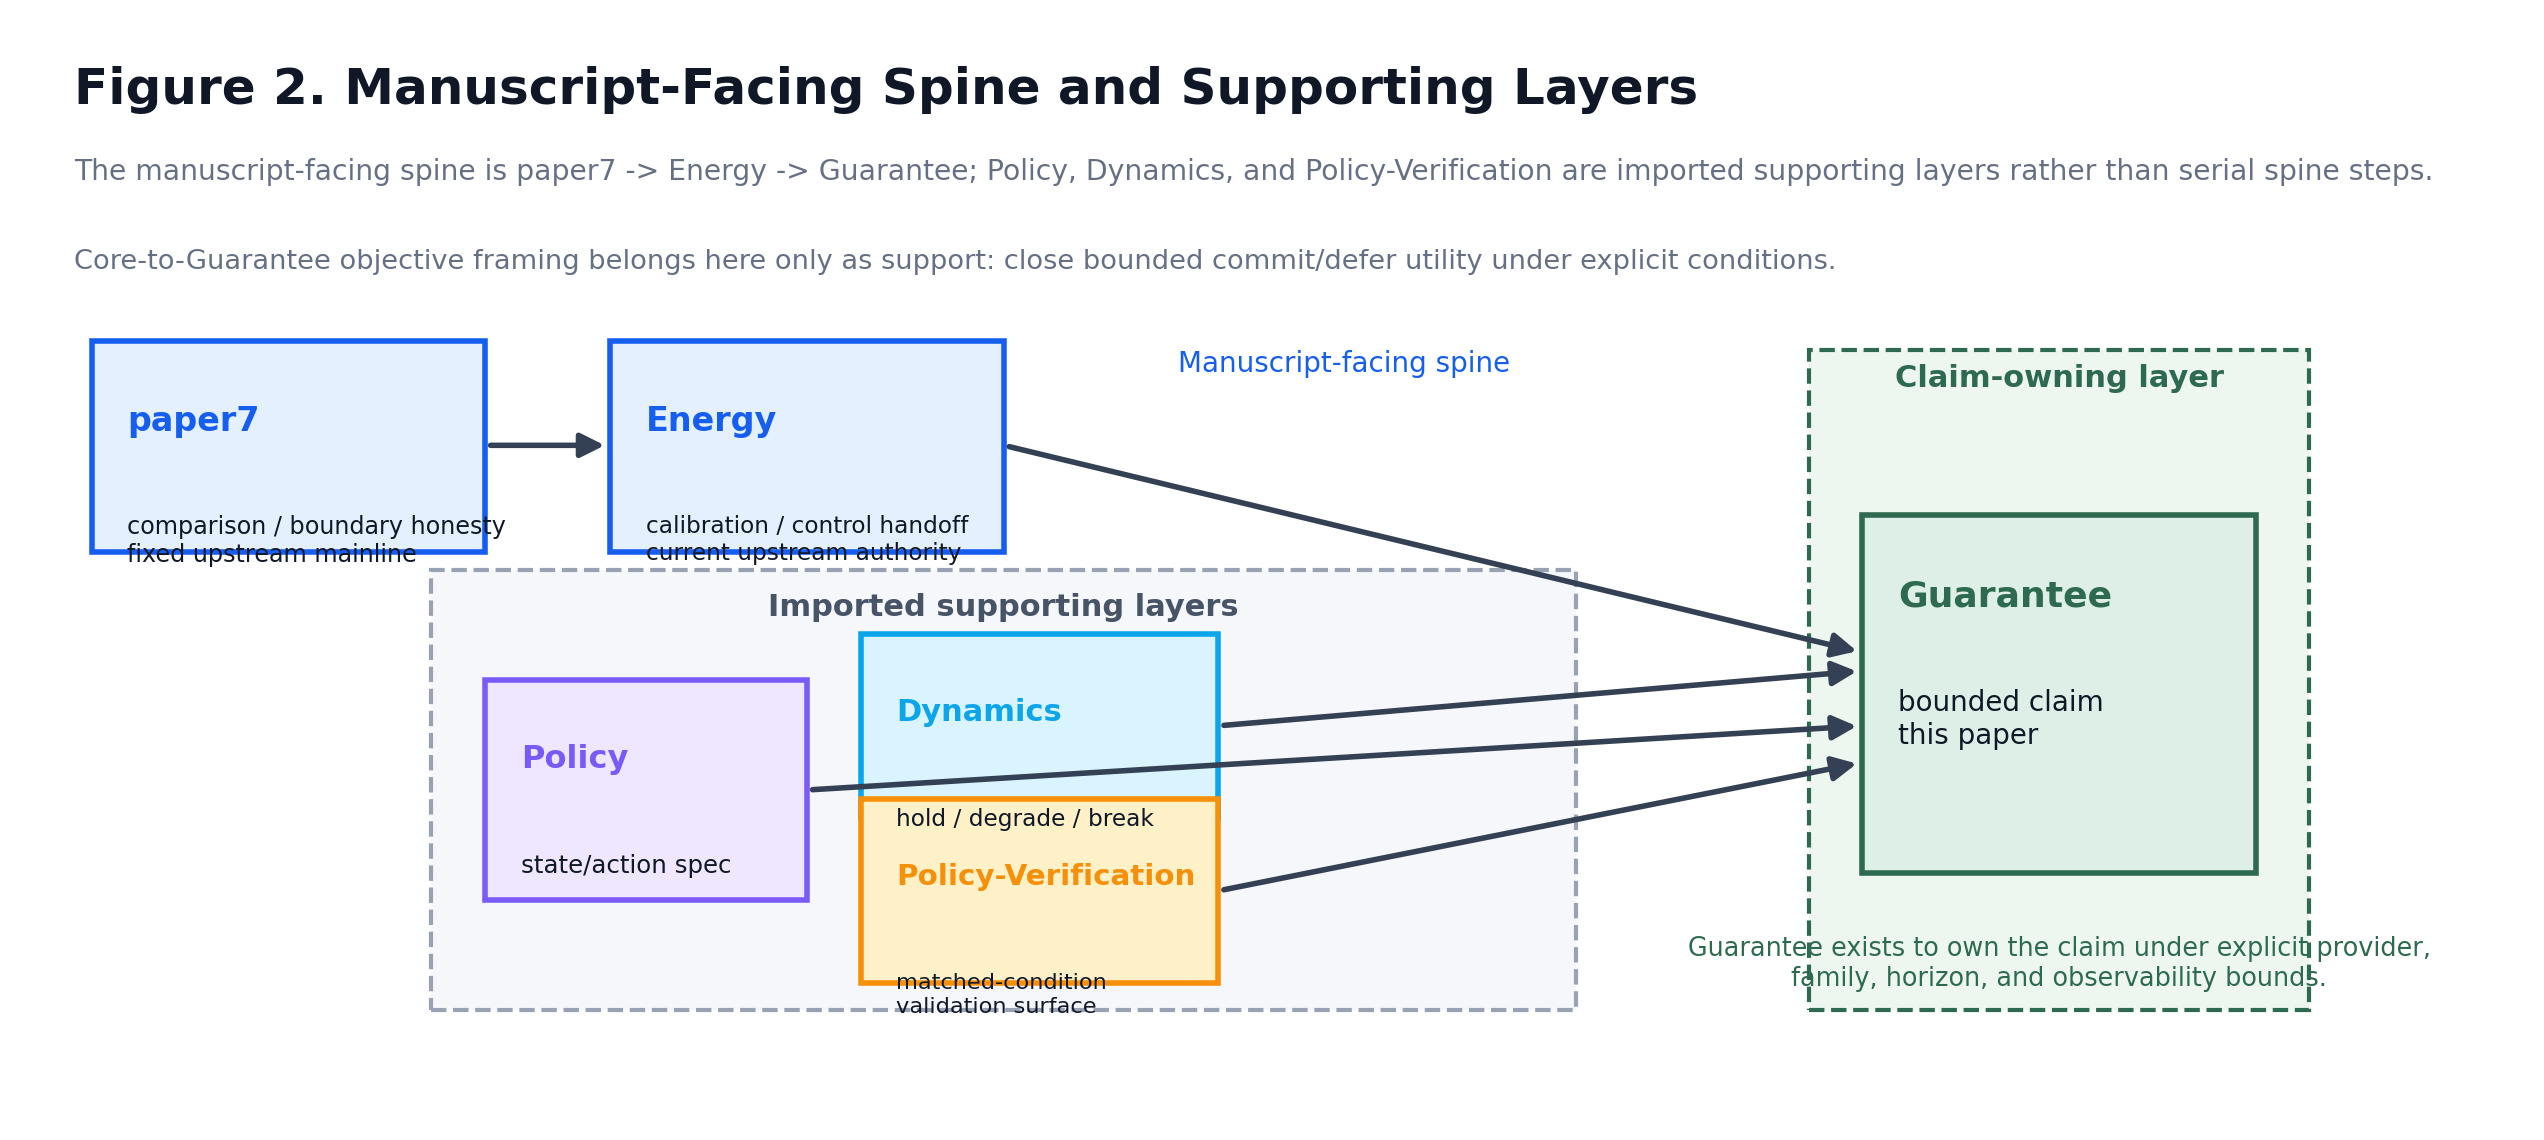
\includegraphics[width=\textwidth]{fig2_guarantee_centered_architecture_v1.png}
\caption{Guarantee-centered downstream architecture. \texttt{Policy},
\texttt{Dynamics}, and \texttt{Policy-Verification} remain supporting layers,
while \texttt{Guarantee} is the current claim-owning paper surface. The broader
Core-to-Guarantee objective is only supportive framing here; this figure's main
purpose is to fix the current ownership split.}
\end{figure}

\section{Supporting-Layer Inputs}

\subsection{Policy Input}

The current policy layer fixes the downstream state vocabulary
(\texttt{active\_objective}, \texttt{suspended\_objective},
\texttt{accepted\_direction}, \texttt{unresolved\_relation},
\texttt{quarantine}, \texttt{local\_relation\_block}) together with the minimal
commit/defer action set. The \texttt{Guarantee} line inherits this vocabulary as
its operating language and does not redesign it locally.

That vocabulary is not ornamental. The early ambiguity-turn surface is the
cleanest current instance of \texttt{defer\_with\_resolution}: no content work
should begin before a direction is accepted, and no unilateral priority choice
should be made on the user's behalf. The downstream acceptance surface is the
current instance of \texttt{commit\_to\_accepted\_direction} in which the
honest carry-forward read is a two-provider mixed result
(\texttt{Anthropic = inconclusive}, \texttt{Gemini = support}) rather than
broad downstream closure. The
repaired first-step side-topic surface is the clearest
first-step instance of \texttt{accepted\_direction} becoming
\texttt{active\_objective} while the prior line is held as
\texttt{suspended\_objective} under \texttt{quarantine}. The later-horizon
boundary then marks the point where \texttt{unresolved\_relation} handling
weakens and \texttt{local\_relation\_block} is no longer treated conservatively.

\subsection{Dynamics Input}

The current dynamics layer contributes mechanism vocabulary only. Its role is to
name where the inherited policy state holds, weakens, or breaks across later
checkpoints. In the current branch, the key motifs are \textit{Stable
Resolution}, \textit{Clean Quarantine Hold}, \textit{Useful Continuation Hold},
\textit{Relation-Preservation Hold}, \textit{Premature Relation Collapse},
\textit{Repeated-Starter Attractor}, \textit{Generic Stall}, and
\textit{Quarantine Leak}.

Using that vocabulary makes the manuscript read as one bounded progression rather
than as three disconnected pilot wins. The ambiguity-turn result is the clearest
instance of \textit{Stable Resolution}. The repaired first-step side-topic result
is the clearest instance of \textit{Clean Quarantine Hold}. The downstream
acceptance result remains narrower: it closes as a two-provider mixed result,
with Anthropic inconclusive and Gemini supportive, so that surface should not
yet be collapsed into uniform \textit{Useful Continuation Hold}. The later-horizon
boundary is best read as weakening \textit{Relation-Preservation Hold} before
\textit{Premature Relation Collapse} appears, with more local residual forms such
as \textit{Generic Stall} or \textit{Repeated-Starter Attractor} where the
template/provider slice warrants them.

\subsection{Policy-Verification Input}

The current policy-verification layer fixes the protocol rules that any prospective
\texttt{baseline vs Energy policy} comparison must satisfy before guarantee text is
allowed. This includes matched-condition comparison, pre-frozen claim units, narrow
family selection, explicit horizon bands, and main-text reporting of both gains and
failure boundaries.

\section{Claim Unit And Boundary Discipline}

Any later guarantee statement in this paper must fill a single bounded claim unit
with the following fields:

\begin{enumerate}
\item provider scope
\item family scope
\item horizon scope
\item observability scope
\item comparison scope
\item supported behavior
\item explicit failure boundary
\item unsupported extension
\end{enumerate}

No guarantee statement is valid if any field is omitted. This paper therefore
inherits the current schema rule that the claim surface must be chosen before
outcome inspection and must remain narrow enough to prevent provider-universal,
family-universal, or long-horizon overreach.

\begin{table}[ht]
\centering
\begin{tabular}{|p{0.13\textwidth}|p{0.27\textwidth}|p{0.22\textwidth}|p{0.24\textwidth}|}
\hline
\textbf{Unit} & \textbf{Scope} & \textbf{Supported behavior} & \textbf{Boundary kept explicit} \\
\hline
Early ambiguity-turn & Tested provider pair, frozen priority-resolution family, early decision boundary & Non-unilateral priority resolution & No downstream acceptance, side-topic/quarantine, or later-horizon extension \\
\hline
Downstream acceptance boundary & Tested provider pair, repaired downstream-acceptance family, first accepted-direction boundary & Two-provider mixed result: Anthropic inconclusive, Gemini support & Do not collapse the mixed result into pair-wide or provider-universal downstream-guarantee language \\
\hline
First-step side-topic/quarantine & Tested provider pair, repaired side-topic family, first accepted side-topic workstart checkpoint & Clean first-step side-topic workstart under explicit side-first acceptance & Incremental lift remains template-bounded and does not authorize later-horizon stability \\
\hline
Later-horizon boundary & Measured later checkpoints only & No additional supported guarantee claim & Failure appears as weakening relation preservation and premature relation collapse, especially on \texttt{C\_incident\_response} at \texttt{turn9} \\
\hline
\end{tabular}
\caption{Current bounded claim surface and explicit boundary discipline in
\texttt{Guarantee}.}
\end{table}

\begin{figure}[ht]
\centering
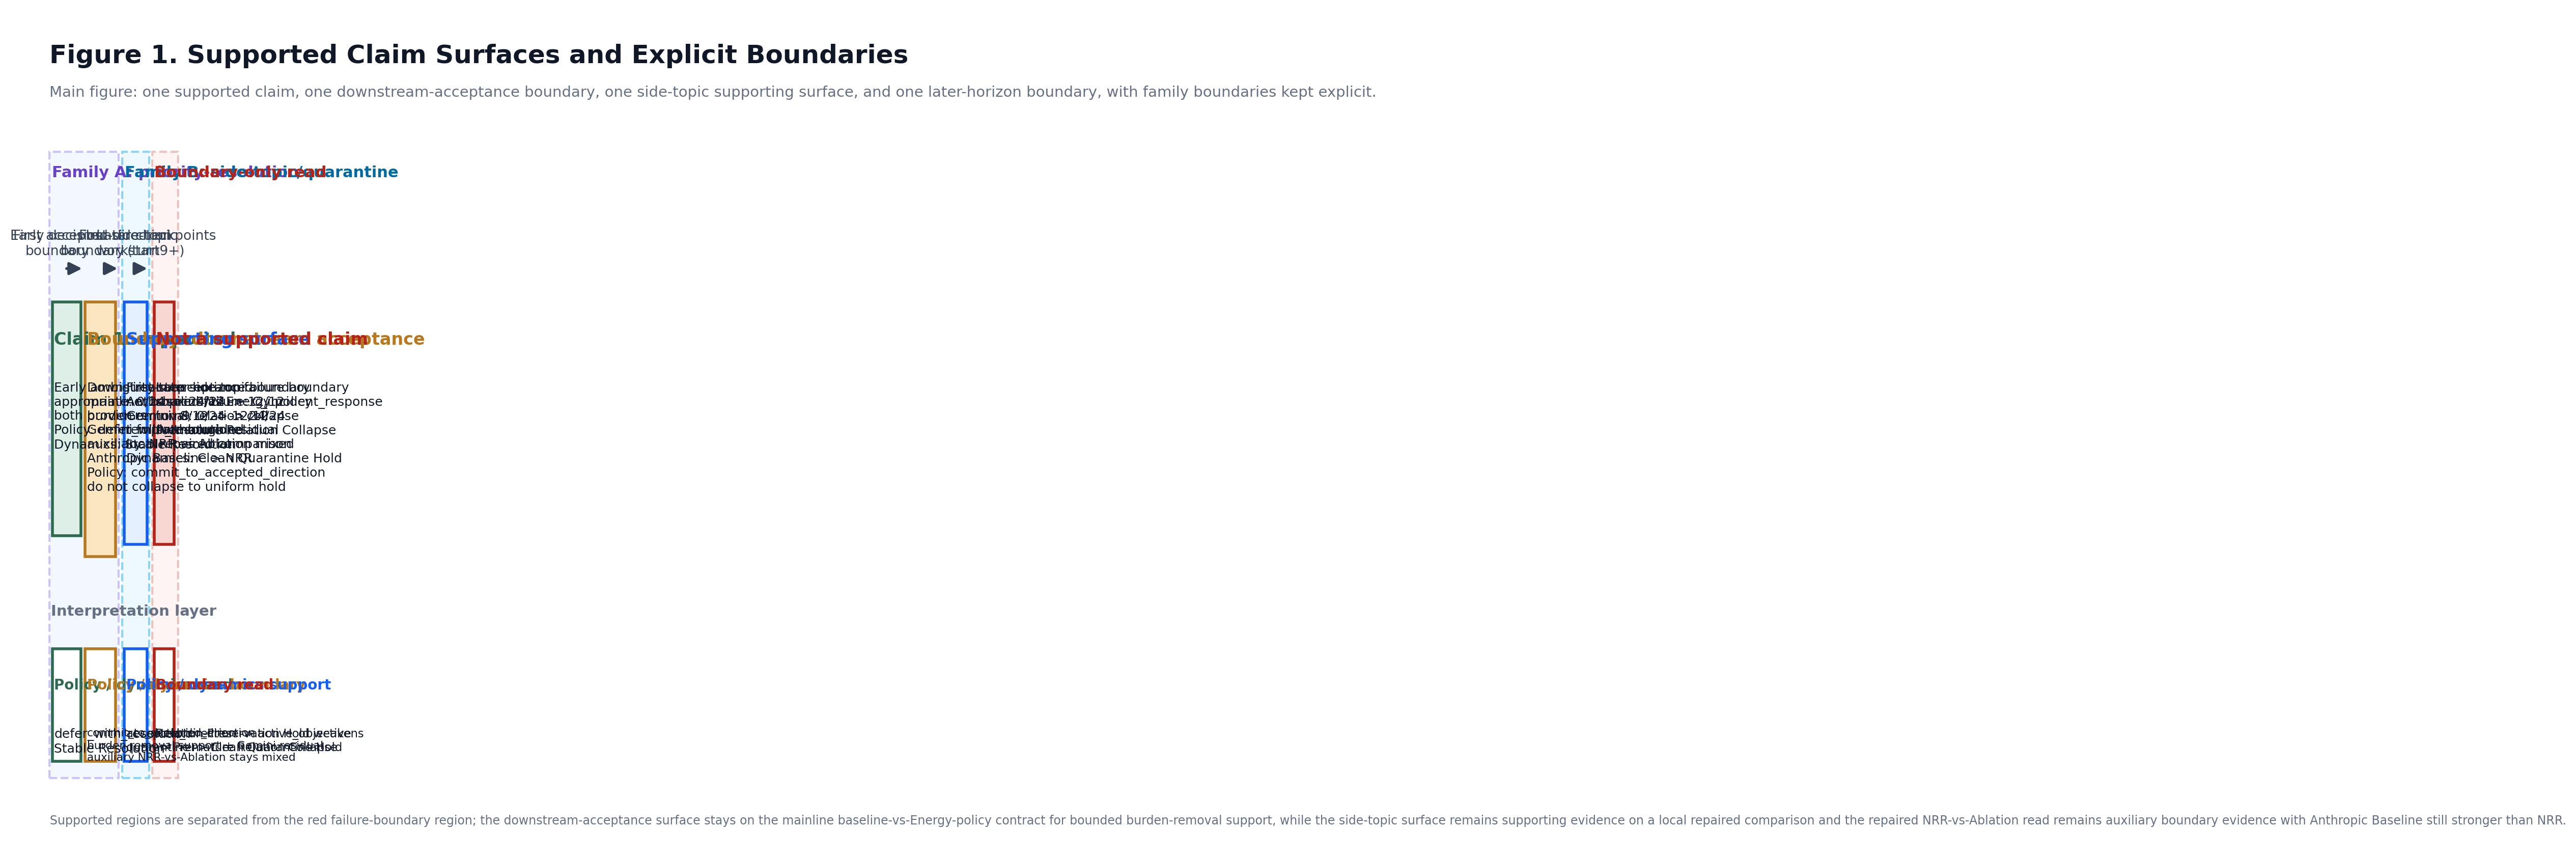
\includegraphics[width=\textwidth]{fig1_supported_claim_progression_v1.png}
\caption{Supported claim progression and explicit failure boundary. Claim 1 and
Claim 2 occupy different horizon points within the same
\texttt{priority-resolution} family, while Claim 3 belongs to the separate
first-step side-topic/quarantine family. The later-horizon region is shown as a
boundary-only read rather than as an additional supported claim.}
\end{figure}

\subsection{First Filled Claim Unit}

The first explicit claim unit in the current manuscript is:

\begin{itemize}
\item provider scope:
  the tested provider pair only (\texttt{claude-sonnet-4-6} and
  \texttt{gemini-2.0-flash})
\item family scope:
  the frozen \texttt{priority-resolution} ambiguity-turn family only
\item horizon scope:
  the early decision boundary only
\item observability scope:
  \texttt{resolution\_attempt\_present},
  \texttt{unilateral\_commit\_absent}, and \texttt{appropriate}
\item comparison scope:
  matched baseline vs Energy-policy under the frozen early
  ambiguity-turn pilot conditions
\item supported behavior:
  non-unilateral priority resolution
\item explicit failure boundary:
  no downstream acceptance, side-topic/quarantine, or later-horizon closure is
  established by this fill
\item unsupported extension:
  no provider-universal, long-horizon, or broad downstream-quality claim is
  authorized
\end{itemize}

In manuscript form, the bounded claim is:

\begin{quote}
Under the tested provider pair, for the frozen \texttt{priority-resolution}
ambiguity-turn family, at the early decision boundary, and on the directly scored
fields \texttt{resolution\_attempt\_present},
\texttt{unilateral\_commit\_absent}, and \texttt{appropriate}, the Energy-policy
arm is supported relative to matched baseline only for non-unilateral priority
resolution. This support excludes downstream acceptance, side-topic/quarantine,
and later-horizon behavior, and it does not extend to provider-universal or broad
downstream-quality claims.
\end{quote}

\subsection{Second Filled Claim Unit}

The second explicit claim unit in the current manuscript is:

\begin{itemize}
\item provider scope:
  the tested provider pair only (\texttt{claude-sonnet-4-6} and
  \texttt{gemini-2.0-flash})
\item family scope:
  the repaired downstream-acceptance family only
\item horizon scope:
  the first accepted-direction downstream boundary only
\item observability scope:
  \texttt{accepted\_direction\_followthrough\_present},
  \texttt{rejected\_direction\_intrusion\_absent},
  \texttt{preacceptance\_rework\_burden\_absent}, and \texttt{appropriate}
\item comparison scope:
  the repaired Phase 2 downstream-acceptance readout under the frozen
  provider-first rule
\item supported behavior:
  two-provider mixed result:
  Anthropic remains `inconclusive` while Gemini reaches `support`
\item explicit failure boundary:
  the surface does not close as pair-wide support, provider-universal
  downstream quality, or later-horizon continuation stability
\item unsupported extension:
  no pair-wide downstream-acceptance guarantee, explicit quarantine closure, or
  later-horizon stability claim is authorized
\end{itemize}

In manuscript form, the bounded claim is:

\begin{quote}
Under the tested provider pair, for the repaired downstream-acceptance family,
at the first accepted-direction downstream boundary, and on the directly scored
fields
\texttt{accepted\_direction\_followthrough\_present},
\texttt{rejected\_direction\_intrusion\_absent},
\texttt{preacceptance\_rework\_burden\_absent}, and \texttt{appropriate}, the
current repaired read closes as a two-provider mixed result rather than as a
pair-wide uniform outcome: Anthropic remains inconclusive while Gemini reaches
support. This surface is therefore carried forward only as a bounded
downstream-acceptance result, not as a pair-wide downstream guarantee, explicit
quarantine closure, or later-horizon stability claim.
\end{quote}

\subsection{Third Filled Claim Unit}

The third explicit claim unit in the current manuscript is:

\begin{itemize}
\item provider scope:
  the tested provider pair only (\texttt{claude-sonnet-4-6} and
  \texttt{gemini-2.0-flash})
\item family scope:
  the repaired first-step side-topic / quarantine family only
\item horizon scope:
  the first accepted side-topic workstart checkpoint only
\item observability scope:
  \texttt{chosen\_side\_direction\_workstart\_present},
  \texttt{suspended\_main\_reference\_absent},
  \texttt{main\_direction\_intrusion\_absent}, and \texttt{appropriate}
\item comparison scope:
  matched baseline vs revised Energy-policy under the repaired first-step
  side-topic / quarantine pilot conditions
\item supported behavior:
  clean first-step side-topic workstart under explicit side-first acceptance
\item explicit failure boundary:
  the gain is incremental rather than a rescue from total baseline failure, and
  the main lift over baseline is concentrated in \texttt{C\_incident\_response}
\item unsupported extension:
  no provider-universal side-topic commitment, uniform template lift, or later-
  horizon side-topic stability claim is authorized
\end{itemize}

In manuscript form, the bounded claim is:

\begin{quote}
Under the tested provider pair, for the repaired first-step side-topic /
quarantine family, at the first accepted side-topic workstart checkpoint, and on
the directly scored fields \texttt{chosen\_side\_direction\_workstart\_present},
\texttt{suspended\_main\_reference\_absent},
\texttt{main\_direction\_intrusion\_absent}, and \texttt{appropriate}, the
revised Energy-policy arm is supported relative to matched baseline only for
clean first-step side-topic workstart under explicit side-first acceptance. This
support excludes provider-universal side-topic commitment, uniform template
lift, and later-horizon side-topic stability, and it remains bounded by the
fact that the main incremental lift over baseline is concentrated in
\texttt{C\_incident\_response}.
\end{quote}

\section{Evidence Import Surface}

The manuscript's imported evidence sources are bundled under
\texttt{supporting\_layer\_sources/current/} so the cited policy, dynamics,
and policy-verification inputs remain directly traceable from the repository:

\begin{itemize}
\item Program design:
  \texttt{energy\_to\_guarantee\_program\_design\_brief\_v1\_2026-03-17.md}
\item Policy:
  \texttt{policy\_minimal\_spec\_current\_v1\_2026-03-18.md}
\item Dynamics:
  \texttt{energy\_dynamics\_mechanism\_skeleton\_candidate\_v2\_2026-03-17.md}
  and
  \texttt{non\_evaluative\_principle\_dynamics\_closure\_note\_v1\_2026-03-19.md}
\item Policy-Verification:
  \texttt{policy\_verification\_pilot\_protocol\_current\_v1\_2026-03-18.md}
\item Guarantee schema:
  \texttt{energy\_guarantee\_claim\_schema\_candidate\_v2\_2026-03-17.md}
\end{itemize}

These inputs are not used to widen the paper into a universality claim. Their
role is to make the bounded claim units traceable while keeping provider,
family, horizon, observability, and failure boundaries explicit.

For ownership-boundary traceability, the same source bundle also carries
\texttt{energy\_to\_policy\_handoff\_memo\_v1\_2026-03-18.md}. That handoff memo
was frozen against the Energy manuscript's then-current \texttt{v8} package.
The now-closed Energy package is at \texttt{v9}, but that later manuscript
revision does not change the downstream support-layer boundaries imported here.

\subsection{First Evidence Import}

The strongest current entry point for the \texttt{Guarantee} line is the frozen
early ambiguity-turn pilot. Under matched baseline vs Energy-policy conditions,
both tested provider slices moved from \texttt{0 / 24} to \texttt{24 / 24} on the
pilot's \texttt{appropriate} field, while baseline failure modes remained visible
as either ambiguity-preserving but unresolved responses or
unilateral/content-before-resolution behavior. The externally cross-checked
carry-forward read is therefore that the Energy-policy surface supports
non-unilateral priority resolution at the early decision boundary on the tested
provider pair. This is a bounded early-control claim only; it does not by itself
establish downstream followthrough, quarantine behavior, later-horizon stability,
or provider-universal validity.

\subsection{Second Evidence Import}

The repaired downstream-acceptance surface is the current second
\texttt{Guarantee} entry point. On the externally closed Phase 2 readout,
Anthropic remains inconclusive while Gemini reaches support, so the truthful
carry-forward read is a two-provider mixed result rather than a pair-wide
uniform outcome. This surface therefore remains manuscript-useful only as
bounded downstream-acceptance reporting under explicit provider sensitivity. It
does not yet license pair-wide downstream guarantee language, explicit
quarantine closure, or later-horizon stability claims.

\subsection{Third Evidence Import}

The third supportable \texttt{Guarantee} entry point is the repaired first-step
side-topic / quarantine pilot. Under matched baseline vs revised Energy-policy
conditions, the revised arm reached \texttt{appropriate = 12 / 12} in both
provider slices, but the honest read is incremental rather than global:
baseline was already fairly strong on \texttt{A\_trip\_planning} and
\texttt{B\_hiring\_packet}, and the main lift over baseline concentrated in
\texttt{C\_incident\_response} (\texttt{1 / 4 -> 4 / 4} on Anthropic and
\texttt{0 / 4 -> 4 / 4} on Gemini). The carry-forward read is therefore a
bounded first-step side-topic workstart claim under explicit side-first
acceptance, not a universal side-topic/quarantine or later-horizon stability
claim.

\begin{table}[ht]
\centering
\begin{tabular}{|p{0.17\textwidth}|p{0.18\textwidth}|p{0.15\textwidth}|p{0.28\textwidth}|}
\hline
\textbf{Surface} & \textbf{Provider scope} & \textbf{Horizon scope} & \textbf{Direct observability scope} \\
\hline
Early ambiguity-turn & Tested provider pair (\texttt{claude-sonnet-4-6}, \texttt{gemini-2.0-flash}) & Early decision boundary & \texttt{resolution\_attempt\_present}, \texttt{unilateral\_commit\_absent}, \texttt{appropriate} \\
\hline
Downstream acceptance boundary & Tested provider pair (\texttt{claude-sonnet-4-6}, \texttt{gemini-2.0-flash}) & First accepted-direction downstream boundary & \texttt{accepted\_direction\_followthrough\_present}, \texttt{rejected\_direction\_intrusion\_absent}, \texttt{preacceptance\_rework\_burden\_absent}, \texttt{appropriate} \\
\hline
First-step side-topic / quarantine & Tested provider pair (\texttt{claude-sonnet-4-6}, \texttt{gemini-2.0-flash}) & First accepted side-topic workstart checkpoint & \texttt{chosen\_side\_direction\_workstart\_present}, \texttt{suspended\_main\_reference\_absent}, \texttt{main\_direction\_intrusion\_absent}, \texttt{appropriate} \\
\hline
Later-horizon boundary & Tested provider pair (\texttt{claude-sonnet-4-6}, \texttt{gemini-2.0-flash}) & Measured later checkpoints, especially \texttt{turn9} & Relation-preservation failure surfaces, most clearly unresolved-relation collapse on \texttt{C\_incident\_response} \\
\hline
\end{tabular}
\caption{Exact tested scope carried forward into the current \texttt{Guarantee}
manuscript.}
\end{table}

\begin{table}[ht]
\centering
\begin{tabular}{|p{0.13\textwidth}|p{0.18\textwidth}|p{0.17\textwidth}|p{0.2\textwidth}|p{0.16\textwidth}|}
\hline
\textbf{Surface} & \textbf{Primary source artifact} & \textbf{Direct observability fields} & \textbf{Supported behavior in this paper} & \textbf{Boundary kept explicit} \\
\hline
Early ambiguity-turn & \texttt{guarantee\_first\_claim\_unit\_fill\_v1\_2026-03-20.md} & \texttt{resolution\_attempt\_present}, \texttt{unilateral\_commit\_absent}, \texttt{appropriate} & Non-unilateral priority resolution at the early decision boundary & No downstream acceptance, side-topic/quarantine, or later-horizon extension \\
\hline
Downstream acceptance boundary & \texttt{guarantee\_second\_claim\_unit\_fill\_v3\_2026-03-21.md} & \texttt{accepted\_direction\_followthrough\_present}, \texttt{rejected\_direction\_intrusion\_absent}, \texttt{preacceptance\_rework\_burden\_absent}, \texttt{appropriate} & Two-provider mixed downstream-acceptance result & Do not collapse the mixed result into pair-wide or provider-universal downstream-guarantee language \\
\hline
First-step side-topic / quarantine & \texttt{guarantee\_third\_claim\_unit\_fill\_v1\_2026-03-20.md} & \texttt{chosen\_side\_direction\_workstart\_present}, \texttt{suspended\_main\_reference\_absent}, \texttt{main\_direction\_intrusion\_absent}, \texttt{appropriate} & Clean first-step side-topic workstart under explicit side-first acceptance & Lift remains template-bounded, with strongest gain on \texttt{C\_incident\_response} \\
\hline
Later-horizon boundary & \texttt{guarantee\_later\_horizon\_failure\_boundary\_v1\_2026-03-20.md} & Relation-preservation failure surfaces at later checkpoints, especially \texttt{turn9} & No additional supported guarantee claim & Preserve later-horizon material as failure-boundary reporting only \\
\hline
\end{tabular}
\caption{Source-to-claim trace for the bounded surfaces carried by the current
\texttt{Guarantee} manuscript.}
\end{table}

\subsection{Policy/Dynamics Interpretation Layer}

Taken together, these supported surfaces define a bounded progression rather than
a universal recipe. At the earliest boundary, the supported behavior is
\texttt{defer\_with\_resolution} and the corresponding dynamics motif is
\textit{Stable Resolution}. At the downstream acceptance boundary, the repaired
read closes as a two-provider mixed result: Anthropic remains inconclusive
while Gemini reaches support, so this surface cannot yet be read as pair-wide
\textit{Useful Continuation Hold}. At the repaired first-step
side-topic boundary, the supported behavior is a clean transition from
\texttt{accepted\_direction} into \texttt{active\_objective} with
\texttt{suspended\_objective} still held in quarantine, which corresponds to
\textit{Clean Quarantine Hold}. The later-horizon limit then becomes easier to
state precisely: the first broad break is not simple suspended-main reactivation
but weakening \textit{Relation-Preservation Hold} until \textit{Premature
Relation Collapse} appears.

\begin{table}[ht]
\centering
\begin{tabular}{|p{0.18\textwidth}|p{0.22\textwidth}|p{0.22\textwidth}|p{0.2\textwidth}|}
\hline
\textbf{Surface} & \textbf{Anthropic-side read} & \textbf{Gemini-side read} & \textbf{Boundary implication} \\
\hline
Early ambiguity-turn & Clean support on the tested early surface & Clean support on the tested early surface & Safe to state only a bounded early-control claim, not broader downstream closure \\
\hline
Downstream acceptance boundary & Inconclusive on the repaired downstream-acceptance surface & Support on the repaired downstream-acceptance surface & Treat the result as a two-provider mixed result, not pair-wide downstream-guarantee language \\
\hline
First-step side-topic / quarantine & Lift is visible, with strongest incremental gain on \texttt{C\_incident\_response} & Lift is also visible, again with the main gain concentrated on \texttt{C\_incident\_response} & Treat the result as template-bounded improvement, not uniform side-topic stability \\
\hline
Later-horizon boundary & Degradation remains visible at later checkpoints & Degradation remains visible at later checkpoints & Preserve later-horizon text as boundary reporting rather than a fourth supported guarantee \\
\hline
\end{tabular}
\caption{Provider-specific residual structure that keeps the current
\texttt{Guarantee} claims bounded.}
\end{table}

\section{Later-Horizon Failure Boundary}

Later-horizon material does not enter this manuscript as a supported guarantee
claim. The current measured horizon family is reported only to mark where the
supported first-step side-topic surface stops being safe to extend. The limited
fact that the first side-topic switch can survive into the next checkpoint, and
that suspended-main quarantine can still be visible there, is included only to
locate the onset of failure. Later degradation remains real, template-dependent,
and not uniformly distributed across providers.

The clearest shared failure surface is \texttt{C\_incident\_response} at
\texttt{turn9}, where both providers tend to collapse the still unresolved
relation by prematurely committing an ordering between \texttt{impact} and
\texttt{root cause}. The correct read is therefore that later-horizon
instability emerges through weakening relation preservation before
suspended-main quarantine itself breaks. This later-horizon material is a
boundary on the current supported surfaces, not an additional supported
\texttt{Guarantee} claim.

\section{Reproducibility And Repository Surface}

The repository surface for this manuscript is intentionally narrow but
self-contained:
\begin{itemize}
\item a current TeX source
\item a current PDF snapshot
\item a working drafting outline
\item a supporting-layer evidence map
\item bounded claim-unit drafting memos
\item a later-horizon failure-boundary memo
\item a policy/dynamics manuscript-integration memo
\item a bundled supporting-layer source surface
\item stable build and verification wrappers
\end{itemize}

The repository therefore exposes both the manuscript-facing claim surface and
the specific imported source layer used to justify it. Checksum verification
executes on the tracked current artifact set, and the documented build wrapper
produces a current PDF in this environment through a source-rendered fallback
when cached TeX resources are incomplete. Full typeset reproduction therefore
remains environment-dependent here, but the bundled repository surface is
organized so the bounded claim surface and its support sources can be inspected
without workspace-only links.

\section{Discussion}

The non-evaluative principle should enter this line as bounded engineering
discipline rather than theorem inflation. In the current read, the practical issue
is not simply whether unresolved content exists, but whether later interaction
forces premature relation collapse while the interaction is still in a retained
state. The \texttt{Guarantee} paper is the correct place to express that read as
a bounded downstream claim surface. In that sense, the manuscript is adjacent to
prior mixed-initiative, clarification, and grounding work, but its objective is
different: it does not primarily propose a better question-asking heuristic or a
general dialogue-success policy. Instead, it asks which bounded commit/defer
claims remain supportable under explicit provider, family, horizon, and
observability restrictions~\cite{chucarroll2000mimic,deboni2003clarification,rao2018evpi,benotti2021grounding}.

The current manuscript line also remains deliberately narrow. It is based on
two tested provider slices, three bounded downstream families, and one later-
horizon boundary read rather than on a broad cross-provider or long-horizon
guarantee. Those limits are not defects to be hidden: they are part of the
bounded-claim discipline that keeps the manuscript from overstating what the
current evidence surface can support.

This staging matters for how the current line should be read. The manuscript is
not claiming a monotone march from early failure to pair-wide downstream
success. The truthful sequence is narrower: the earlier Phase 1 surface remains
provider-first \texttt{non-support}, while the current downstream-acceptance
surface closes only as a two-provider mixed result, with Anthropic still
\texttt{inconclusive} and Gemini reaching \texttt{support}. That asymmetry is
not noise to be hidden or a reason to over-weight one provider slice. It is the
current bounded result.

\section{Conclusion}

This version establishes a bounded manuscript surface for \texttt{Guarantee}.
It fixes the downstream ownership split, consolidates two supported claim units
for the early ambiguity-turn surface and the repaired first-step side-topic/
quarantine surface, carries the repaired downstream-acceptance surface forward
as a two-provider mixed result, and keeps the later-horizon limit explicit as
failure-boundary reporting rather than as a further supported claim. It also
ties those supported and unsupported regions directly to the inherited policy
vocabulary and dynamics motifs without promoting the line into
provider-universal, family-universal, or theorem-level language. In practical
terms, the current \texttt{Guarantee} line closes this pass around a staged
bounded result: Phase 1 remains \texttt{non-support}, and Phase 2 remains a
two-provider mixed result rather than a pair-wide downstream guarantee. What
remains outside the present claim surface is broader provider coverage, broader
downstream family coverage, and later-horizon closure.

\begin{thebibliography}{99}
\raggedright

\bibitem{saito2025nrr}
K.~Saito,
\newblock ``NRR-Core: Non-Resolution Reasoning as a Computational Framework for Contextual Identity and Ambiguity Preservation,''
\newblock \emph{arXiv preprint arXiv:2512.13478}, 2025.

\bibitem{saito2026phi}
K.~Saito,
\newblock ``NRR-Phi: Text-to-State Mapping for Ambiguity Preservation in LLM Inference,''
\newblock \emph{arXiv preprint arXiv:2601.19933}, 2026.

\bibitem{saito2026ime}
K.~Saito,
\newblock ``NRR-IME: Interface Decomposition for Stable State Transitions on Stateless LLM APIs,''
\newblock GitHub repository: \texttt{https://github.com/kei-saito-research/nrr-ime}; local manuscript snapshot \texttt{paper4-nrr-ime-v67.tex}, commit \texttt{99f5ebb}, 2026.

\bibitem{saito2026transfer}
K.~Saito,
\newblock ``NRR-Transfer: Cross-Domain Transfer of Phase 1.5 Operators Under Fixed Interface Constraints,''
\newblock GitHub repository: \texttt{https://github.com/kei-saito-research/nrr-transfer}; local manuscript snapshot \texttt{paper5-nrr-transfer-v50.tex}, commit \texttt{0c47396}, 2026.

\bibitem{saito2026coupled}
K.~Saito,
\newblock ``NRR-Coupled (cp): Dependency-Consistency Evaluation for Coupled State Updates,''
\newblock GitHub repository: \texttt{https://github.com/kei-saito-research/nrr-coupled}; local manuscript snapshot \texttt{paper6-nrr-coupled-v19.tex}, commit \texttt{10d9e35}, 2026.

\bibitem{saito2026principles}
K.~Saito,
\newblock ``NRR-Principles: Computational Efficiency Through Delayed Commitment in Stateful LLM Systems,''
\newblock GitHub repository: \texttt{https://github.com/kei-saito-research/nrr-principles}; local manuscript snapshot \texttt{nrr-principles_manuscript_v11.tex}, commit \texttt{6d901c5}, 2026.

\bibitem{saito2026boundary}
K.~Saito,
\newblock ``NRR-Boundary: Same Operators, Opposite Effects by Provider and Order,''
\newblock GitHub repository: \texttt{https://github.com/kei-saito-research/nrr-boundary}; local manuscript snapshot \texttt{nrr-boundary_manuscript_v22.tex}, commit \texttt{7b911db}, 2026.

\bibitem{saito2026energy}
K.~Saito,
\newblock ``NRR-Energy: Calibration of Commit/Defer Utility Under Existing Paired Boundary Data,''
\newblock Local repository snapshot \texttt{nrr-energy}, current manuscript snapshot \texttt{nrr-energy_manuscript_v9.tex}, local commit \texttt{b82b444}; bundled handoff snapshot \texttt{supporting\_layer\_sources/current/nrr-energy\_manuscript\_v8.tex}, 2026.

\bibitem{chucarroll2000mimic}
J.~Chu-Carroll,
\newblock ``MIMIC: An Adaptive Mixed Initiative Spoken Dialogue System for Information Queries,''
\newblock In \emph{Sixth Applied Natural Language Processing Conference}, pages 97--104, Seattle, Washington, USA, 2000.

\bibitem{deboni2003clarification}
M.~De Boni and S.~Manandhar,
\newblock ``An Analysis of Clarification Dialogue for Question Answering,''
\newblock In \emph{Proceedings of the 2003 Human Language Technology Conference of the North American Chapter of the Association for Computational Linguistics}, pages 48--55, 2003.

\bibitem{saito2017taskdialogue}
T.-H.~Wen, D.~Vandyke, N.~Mrk{\v{s}}i{\'c}, M.~Ga{\v{s}}i{\'c}, L.~M.~Rojas-Barahona, P.-H.~Su, S.~Ultes, and S.~Young,
\newblock ``A Network-based End-to-End Trainable Task-oriented Dialogue System,''
\newblock In \emph{Proceedings of the 15th Conference of the European Chapter of the Association for Computational Linguistics: Volume 1, Long Papers}, pages 438--449, Valencia, Spain, 2017.

\bibitem{rao2018evpi}
S.~Rao and H.~Daum{\'e} III,
\newblock ``Learning to Ask Good Questions: Ranking Clarification Questions using Neural Expected Value of Perfect Information,''
\newblock In \emph{Proceedings of the 56th Annual Meeting of the Association for Computational Linguistics (Volume 1: Long Papers)}, pages 2737--2746, Melbourne, Australia, 2018.

\bibitem{hu2020interactive}
X.~Hu, Z.~Wen, Y.~Wang, X.~Li, and G.~de Melo,
\newblock ``Interactive Question Clarification in Dialogue via Reinforcement Learning,''
\newblock In \emph{Proceedings of the 28th International Conference on Computational Linguistics: Industry Track}, pages 78--89, Online, 2020.

\bibitem{benotti2021groundedclarifications}
L.~Benotti and P.~Blackburn,
\newblock ``A recipe for annotating grounded clarifications,''
\newblock In \emph{Proceedings of the 2021 Conference of the North American Chapter of the Association for Computational Linguistics: Human Language Technologies}, pages 4065--4077, Online, 2021.

\bibitem{benotti2021grounding}
L.~Benotti and P.~Blackburn,
\newblock ``Grounding as a Collaborative Process,''
\newblock In \emph{Proceedings of the 16th Conference of the European Chapter of the Association for Computational Linguistics: Main Volume}, pages 515--531, Online, 2021.

\end{thebibliography}

\end{document}
